\documentclass[tikz,border=10pt]{standalone}
\usepackage{tikz}
\usepackage{tikz-cd}
\usetikzlibrary{arrows,automata,shapes,positioning,decorations.pathmorphing}
% \tikzset{->,>=stealth',auto}
\tikzset{->,auto}
\tikzset{>={Latex[width=2mm,length=2mm]}}
\tikzset{state/.style={shape=circle, draw, fill=white, initial text=,
    inner sep=.5mm, minimum size=2mm}}
\tikzset{state with output/.style={shape=rectangle split, rectangle
    split parts=2, draw, fill=white,
    initial text=, inner sep=1mm}}
\tikzset{every node={font=\footnotesize}}

\begin{document}
  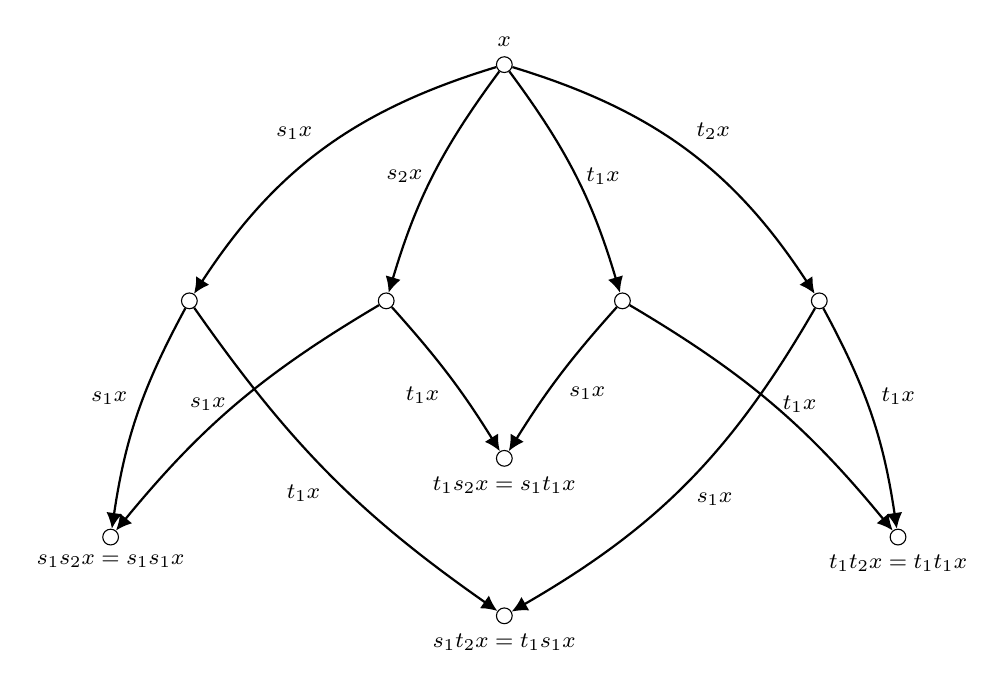
\begin{tikzpicture}[node distance=2cm, align=center]
    \tikzstyle{every node}=[font=\footnotesize]
    \tikzstyle{every state}=[fill=white,shape=circle,inner
    sep=.5mm,minimum size=3mm]
    \title{unfolded HDA}
    
    \node[state] (d11d12) [label=below:{$t_1 t_2x = t_1  t_1x$}] at (-3, -2) {};
    \node[state] (d12) at (-4, 1) {};
    \node[state] (d11d02) [label=below:{$t_1 s_2x = s_1  t_1x$}] at (-8, -1) {};
    \node[state] (d11)at (-6.5,1) {};
    \node[state] (x) [label=above:{$x$}] at (-8, 4) {};
    \node[state] (d02) at (-9.5, 1) {};
    \node[state] (d01) at (-12, 1) {};
    \node[state] (d01d02) [label=below:{$s_1  s_2x = s_1  s_1x$}] at (-13, -2) {};
    \node[state] (d01d12) [label=below:{$s_1  t_2x = t_1  s_1x$}] at (-8,-3) {};
    
    
    \draw [->][draw=black, thick, bend right=20] (x) to node [above left] {$s_1x$} (d01);
    \draw [->][draw=black, thick, bend right=10] (x) to node [left] {$s_2x$} (d02);
    \draw [->][draw=black, thick, bend left=10] (x) to node [right] {$t_1x$} (d11);
    \draw [->][draw=black, thick, bend left=20] (x) to node [above right] {$t_2x$} (d12);
    
    \draw [->][draw=black, thick, bend right=10] (d01) to node [above left] {$s_1x$} (d01d02);
    \draw [->][draw=black, thick, bend right=10] (d01) to node [below left] {$t_1x$} (d01d12);
    
    \draw [->][draw=black, thick, bend right=10] (d02) to node [left] {$s_1x$} (d01d02);
    \draw [->][draw=black, thick, bend left=5] (d02) to node [below left] {$t_1x$} (d11d02);
    
    \draw [->][draw=black, thick, bend right=5] (d11) to node [below right] {$s_1x$} (d11d02);
    \draw [->][draw=black, thick, bend left=10] (d11) to node [right] {$t_1x$} (d11d12);
    
    \draw [->][draw=black, thick, bend left=15] (d12) to node [below right] {$s_1x$} (d01d12);
    \draw [->][draw=black, thick, bend left=10] (d12) to node [above right] {$t_1x$} (d11d12);

  \end{tikzpicture}
\end{document}